\documentclass[journal]{IEEEtran}
\usepackage{amsmath,amsfonts}
\usepackage{algorithm,algpseudocode}
\usepackage{array}
\usepackage[caption=false,font=normalsize,labelfont=sf,textfont=sf]{subfig}
\usepackage{textcomp}
\usepackage{stfloats}
\usepackage{url}
\usepackage{verbatim}
\usepackage{graphicx}
\usepackage[bookmarksnumbered, colorlinks, plainpages]{hyperref}
\usepackage[dvipsnames]{xcolor}
%\hyphenation{op-tical net-works semi-conduc-tor IEEE-Xplore}
\usepackage{balance}
\newcount\myloopcounter

\newcommand{\repeatit}[2][10]{%
  \myloopcounter0% initialize the loop counter
  \loop\ifnum\myloopcounter < #1 % Test if the loop counter is < #1
  #2%
  \advance\myloopcounter by 1 % 
  \repeat % start again
}

\begin{document}
\title{Final Report of the Group Project for CS5351\\
\colorbox{yellow}{\textit{!We Need Project Title: An informative title!}}
}

\input{private/author}


%\markboth{Journal of \LaTeX\ Class Files,~Vol.~18, No.~9, September~2020}%
%{How to Use the IEEEtran \LaTeX \ Templates}

\markboth{Final Report of the Group Project for CS5351, December~2023}%
{Title of the Project TBD.}

\maketitle

\begin{abstract}
This document describes blablabal....
abstract to be consideration.

\textit{Requirements: needs (150 words) }

\end{abstract}

\begin{IEEEkeywords}
Software Engineering, Software Testing, Computer Science, Software Maintainance, Software Debug.
\end{IEEEkeywords}


\section{Introduction}
\IEEEPARstart{T}{his} collaborative effort reflects the team's dedication to creating tools that aid software engineers in improving code quality by detecting code smells. 

The following sections provide an in-depth look at the project's background, the proposed solution, the software development process, evaluation results, and concluding remarks.

\textbf{(about 1-1.5 pages)}

\section{Related Work}
\noindent Web security has become quite important nowdays due to the increase in cybercrimes. Developers are very concerned about how to avoid obvious security issues such as hacking and data breaches, when designing and developing websites. There have been many studies that have proposed many technologies and tools to prevent web security vulnerabilities and defense methods, and there have also been many studies that have evaluated the effectiveness and missed detection probability of existing vulnerability scanning methods. 

Abirami's team created a tool to detect vulnerabilities such as XSS and SQLI using Python language. The program run automatically to send reports to relevant users\cite{9155908}. Zhang's team proposed an automatic detection tool dealing with multiple type of vulnerabilities. The tool includes a combination of three vulnerability detections, including cross-site scripting attacks, SQL injections, and directory operations\cite{8983828}. A web program named Gregorius used AJAX crawling to improve vulnerability detection efficiency\cite{9092613}. There is also a detector named ETSS, which is a versatile and modular online vulnerability detection created by Rocha and Souto that automatically checks web applications for XSS vulnerabilities. It can find and evaluate all data entry points of an application, as well as create code injection tests for each test\cite{6924244}. Web application penetration testing is designed to evaluate the design, configuration, and architecture of a web application. Shebli's group  studied penetration testing processes and tools, focusing on comparing four different port scanning tools to demonstrate their effectiveness\cite{8378035}. In recent years, with the development of machine learning, many web application vulnerability detection methods based on machine learning have emerged. Combined with the development history of machine learning security vulnerability detection technology, Lilan Hu's team designed and implemented a cross-site scripting security vulnerability detection model for web applications, a verification code identification function was added\cite{article10.1088/1742-6596/1827/1/012061}. Calzavara's group proposed a methodology to leverage machine learning for the detection of web application vulnerabilities. They used it in the design of Mitch, the first ML solution for the black-box detection of cross-site request forgery vulnerabilities\cite{8966601}.

\vspace{1em}

\textit{Requirements: Present your fact finding about existing solutions toward solving the problem stated in the section on Introduction}. 

\textbf{(about 1 page)}

\section{Preliminaries}
\noindent The 3rd part is Preliminaries.
blablabal....

The Preliminaries section lays the foundation for the reader by presenting essential technical background information. It encompasses a summary of the knowledge required to understand the developed tools, focusing on code smells, their significance, and existing tools in the domain. This section aims to equip the reader with the necessary context to comprehend the subsequent discussion.

\subsection{Separation of front and back ends}
Front-end and back-end separation is a modern web development architecture, as shown in Fig.\ref{fig:Separation}, and design pattern that separates the front-end interface of the web page from the back-end server application logic, enhancing the maintainability of the application. Since front-end and back-end are independent, we can choose the technology stack that best suits our respective needs. For example, the front-end can use React, Vue.js or Angular, while the back-end can use Node.js, Python's Flask or Django, Ruby on Rails, etc. This separation improves development efficiency because development teams can independently update and extend different parts of the application without interfering with each other.

\begin{figure}[!t]
  \centering
  
\includegraphics[width=2.5in]{figures/Preliminaries1.png}
  \caption{Separation of Front and Back ends}
  \label{fig:Separation}
  \end{figure}

\subsection{React for Front-End Development }
React is an open source JavaScript library widely used for building user interfaces. It allows developers to build applications using a componentized approach, meaning that each part of the user interface is encapsulated into independent, reusable components. React's responsive design principles ensure that the user interface can quickly respond to data changes. Fetch API is used for network requests in React applications. In this project, Fetch is used to communicate with the backend service to retrieve and send data.

\subsection{Ant Design of React}
Antd is a React UI library that follows the Ant Design specification and contains a set of high-quality components and demos for building rich interactive user interfaces.

\subsection{Cross-origin resource sharing}
Cross-origin resource sharing (CORS) is a security mechanism that allows or restricts resources on a web page (such as fonts, JavaScript, etc.) to be accessed by another domain name with a different origin. In the integration of React and Flask, CORS is an important consideration because the frontend and backend are usually deployed on different domains. Corresponding CORS strategies are used in this project to ensure safe and effective front-end and back-end communication.

\subsection{Postman}
Postman is an ideal tool for building and testing APIs. It supports all common HTTP request types, such as GET, POST, PUT, DELETE, etc. It allows users to easily add request parameters, header information, authentication data, etc. Postman provides a user-friendly interface that allows developers to easily send requests to the server and view the responses. By viewing the response data and status codes of the API, developers can quickly locate the problem.

\subsection{Flask for Back-End Development}
Flask is a lightweight web application framework written in Python. It is designed to be easily extensible and provides the necessary tools and features to build reliable web applications. In this project, Flask serves as the back-end framework to handle client requests and interact with the database.

\subsection{Database storage}
This project uses a database to store application data, which may include user information, transaction data, etc. In addition, the system supports file upload functionality, which is crucial for processing user-submitted code files. Flask provides integration with databases and the ability to handle file uploads.

\subsection{Nginx}
Nginx is a high-performance HTTP and reverse proxy server, which can also be used as a mail proxy server. In this project, Nginx is used as the web server, responsible for handling HTTP requests and forwarding them to the Flask application. The use of Nginx improves the reliability and load balancing capabilities of the application.

\subsection{Docker}
Docker is a popular open source containerization platform that allows developers to easily create, deploy, and run applications. By using Docker, developers can package applications and their dependencies into a portable container that can run on any Docker-enabled machine, ensuring application consistency across different environments.

\subsection{Kubernetes}
Kubernetes, also known as K8s, is an open-source container orchestration platform designed to automate the deployment, scaling, and management of containerized applications.  Kubernetes groups containers into logical units called pods, facilitating seamless management and discovery. Its core features include automated scaling, pod orchestration, services for networking, replication controllers, and deployments for ensuring application stability. With a master-node architecture, extensibility through Custom Resource Definitions (CRDs), and a vibrant community, Kubernetes has emerged as the industry standard, streamlining the complexities of containerized application deployment and management.

\textbf{(about 1-2 pages)}

\section{Solution}
\noindent The Solution section articulates the team's approach to addressing code smells using an innovative tool. This part of the report encompasses detailed descriptions, algorithms, figures, and code listings that elucidate the inner workings of the solution. The team provides an example walkthrough to illustrate how the tool functions, emphasizing its relevance to topics covered in the CS5351 course.

\subsection{Cross-Origin Resource Sharing}
Solving cross-domain problems is an important challenge in implementing a front-end and back-end separation architecture. Cross-Origin Resource Sharing (CORS) issues occur when a web page attempts to request resources from different sources (domain names, protocols, or ports). These requests may be rejected due to the browser's same-origin policy restrictions. Here are our ways to resolve cross-domain issues:

\subsubsection{Use CORS Headers}
The most common approach is to implement CORS on the server side. This can be achieved by adding specific CORS headers to the HTTP response. These headers tell the browser to allow web pages from different origins to access the resource. Allowing all sources can lead to security vulnerabilities, so we limit only specific, trusted sources.

\subsubsection{Reverse Proxy server by Nginx}
Using a reverse proxy server between the front-end and back-end can effectively solve cross-domain issues, as shown in Fig.\ref{fig:reversesolution}. The proxy server receives the request sent by the front end and forwards the request to the actual backend server.

\begin{figure}[!t]
  \centering
  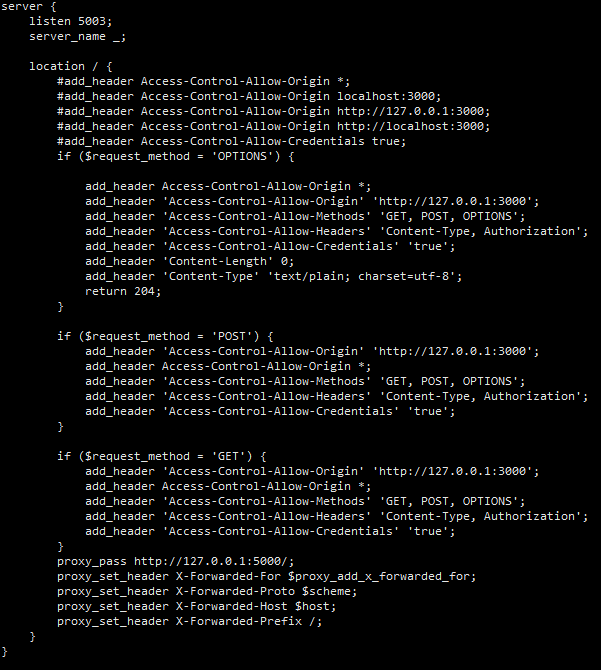
\includegraphics[width=3in]{figures/solution-nginx.png}
  \caption{Reverse Proxy server by Nginx}
  \label{fig:reversesolution}
  \end{figure}

\subsection{Interface adjustment and troubleshooting, communication between front-end and back-end}
During the software engineering process, effective communication between front-end and back-end teams is critical to successfully tuning interfaces. Postman is a powerful tool that can play a key role in this process. The following are the steps to use Postman to communicate with the back-end interface, adjust the interface, and troubleshoot based on the software engineering process:
\subsubsection{Define and understand interface specifications}
\begin{itemize}
  \item Requirements analysis: In the early stages of development, our front-end and back-end teams jointly reviewed functional requirements and clarify the purpose and expected behavior of the interface.
  \item Interface documentation: Backend teams created detailed interface documentation, including endpoint URLs, request methods (GET, POST, etc.), request parameters, expected response formats, and status codes, as shown in Fig.\ref{fig:interfacespec}.
  \item Review and feedback: Our front-end team reviewed these documents and ask questions or request changes.
\end{itemize}

\begin{figure}[!t]
  \centering
  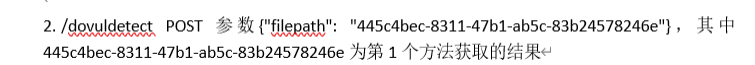
\includegraphics[width=3in]{figures/solution-interspec.png}
  \caption{Interface documentation}
  \label{fig:interfacespec}
  \end{figure}

\subsubsection{Use Postman(Fig.\ref{fig:postman}) for interface testing}
\begin{itemize}
  \item Write a request: According to the interface document, set the URL, method, header, parameters, etc. of the request.
  \item Send a request: Execute the request and observe the response. Check whether the response status code, data structure and data content are as expected.
\end{itemize}

\begin{figure}[!t]
  \centering
  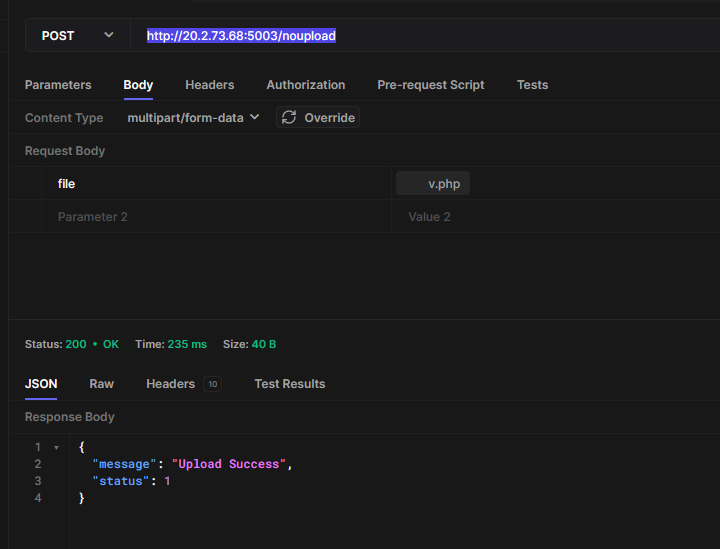
\includegraphics[width=3in]{figures/solution-postman.png}
  \caption{Postman for interface testing}
  \label{fig:postman}
  \end{figure}

\subsubsection{Interface debugging and troubleshooting}
\begin{itemize}
  \item Record and share results: Use Postman's to record and share test results with your backend team, especially when issues were discovered.
  \item Error identification: For error responses, analyze the error message or status code in the response body to determine the nature of the error.
\end{itemize}
\subsubsection{Communication and collaboration}
\begin{itemize}
  \item Feedback and modifications: Feed back the problems discovered during testing to the backend team and discuss how to modify the interface to meet needs.
  \item Update documentation: Once the interface changes, make sure to update the interface documentation to keep the documentation up-to-date.
  \item Iterative testing: Repeat testing of the modified interface to ensure that all issues have been resolved.
\end{itemize}

\begin{figure*} 
  \centering
\subfloat[\label{1a}]{%
     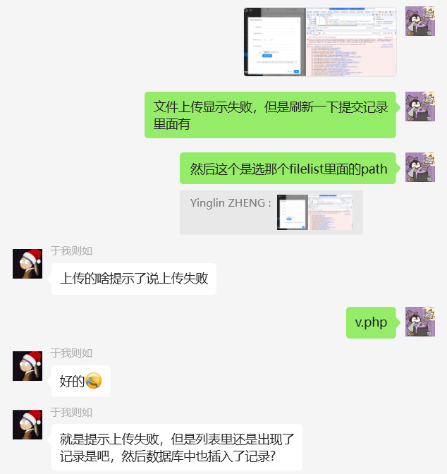
\includegraphics[height=2in,width=0.3\textwidth]{figures/collaboration1.png}}
  \hfill
\subfloat[\label{1b}]{%
      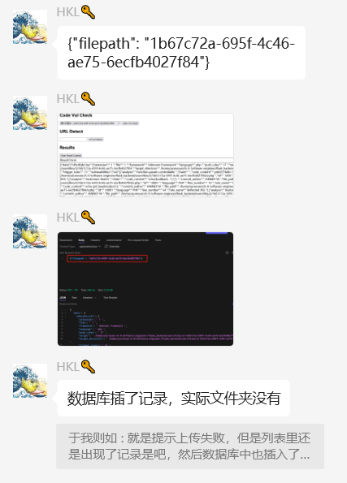
\includegraphics[height=2in,width=0.3\textwidth]{figures/collaboration2.png}}
  \hfill
\subfloat[\label{1c}]{%
      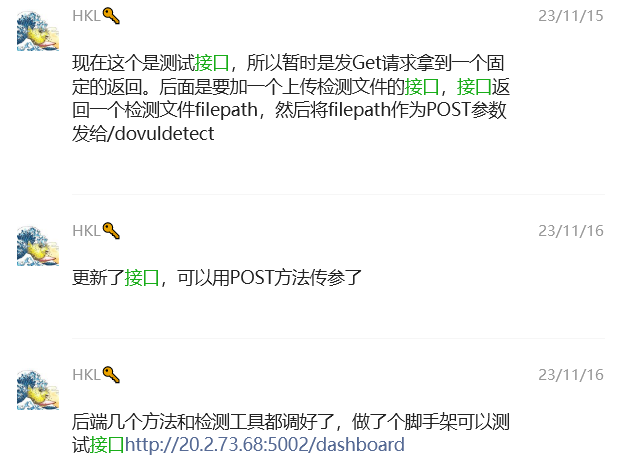
\includegraphics[height=2in,width=0.3\textwidth]{figures/collaboration3.png}}
  \hfill
  \\
\subfloat[\label{1d}]{%
      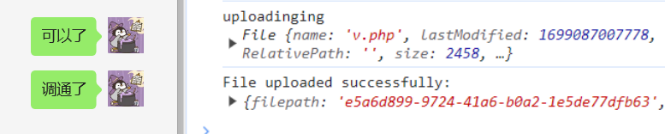
\includegraphics[height=0.8in,width=0.5\textwidth]{figures/collaboration4.png}}
\caption{(a), (b) Feed back the problems discovered during testing to the backend team and discuss how to modify the interface to meet needs.(c) Once the interface changes, make sure to update the interface documentation to keep the documentation up-to-date,(d) Iterative testing: Repeat testing of the modified interface to ensure that all issues have been resolved.}
\label{fig:collaboration} 
\end{figure*}


\subsection{Collaboration between different front-end developers}
In the software engineering process, using Git for version control and branch management is a common practice, especially in projects where multiple people collaborate. The following is the branch strategy of our front-end development team based on Git.
\subsubsection{Create a front-end branch}
Create a development branch (front-end) from the main branch. This branch contains all the latest front-end development work.
\subsubsection{Separate feature branches from the development branch}
Each developer creates his or her own branch (Yinglin-ZHENG, Xi-CHEN, etc.) from the development branch to develop assigned functional tasks or fix bugs, which ensures that development work is independent of each other and reduces conflicts.
\subsubsection{Add Readable commits and Request Review for Merge}
Developers committed their code with readable information and requested review and test from each other's, then wait for other coders to make comment, if the function is completed correctly, it can be merged into front-end branch. If there are something conflict when merge, we made a discussion between the code writers.

\subsection{Deal With JSON Response in front-end}
\subsubsection{Data interaction and analysis}
\begin{itemize}
  \item Receive JSON data: The front end receives a JSON formatted response from the back end. This is achieved by using the Fetch API and processing the response, as shown in Fig.\ref{fig:datainteana1a}.
  \item Parse JSON: The front-end application parses JSON data and converts it into JavaScript objects for further processing and display, as shown in Fig.\ref{fig:datainteana1b}.
\end{itemize}

\begin{figure} 
  \centering
\subfloat[Receive JSON data\label{fig:datainteana1a}]{%
     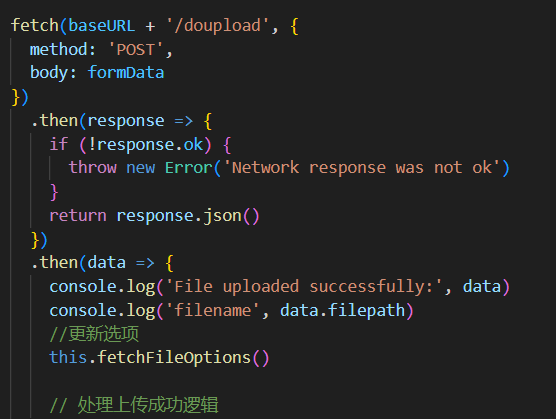
\includegraphics[height=2in,width=0.45\linewidth]{figures/json1.png}}
  \hfill
\subfloat[Parse JSON\label{fig:datainteana1b}]{%
      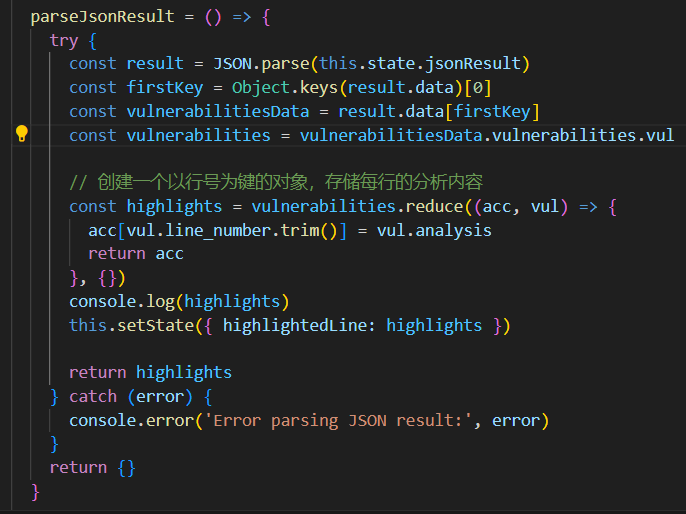
\includegraphics[height=2in,width=0.45\linewidth]{figures/json2.png}}
\caption{Data interaction and analysis}
\label{fig:datainteana} 
\end{figure}

\subsubsection{Front-end interface design}

\begin{itemize}
  \item Display code: Use appropriate HTML elements such as <pre> and <code> tags to display code, as shown in Fig.\ref{fig:displaycode}.
  \item Code highlighting: Use front-end libraries highlight.js, to implement code highlighting, as shown in Fig.\ref{fig:highlightcode}. 
\end{itemize}

\begin{figure}[!t]
  \centering
  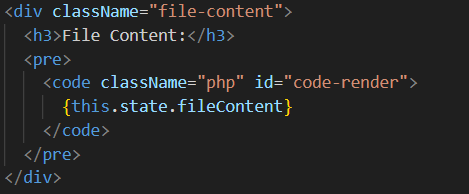
\includegraphics[width=2in]{figures/displaycode.png}
  \caption{Display code}
  \label{fig:displaycode}
  \end{figure}

\begin{figure}[!t]
  \centering
  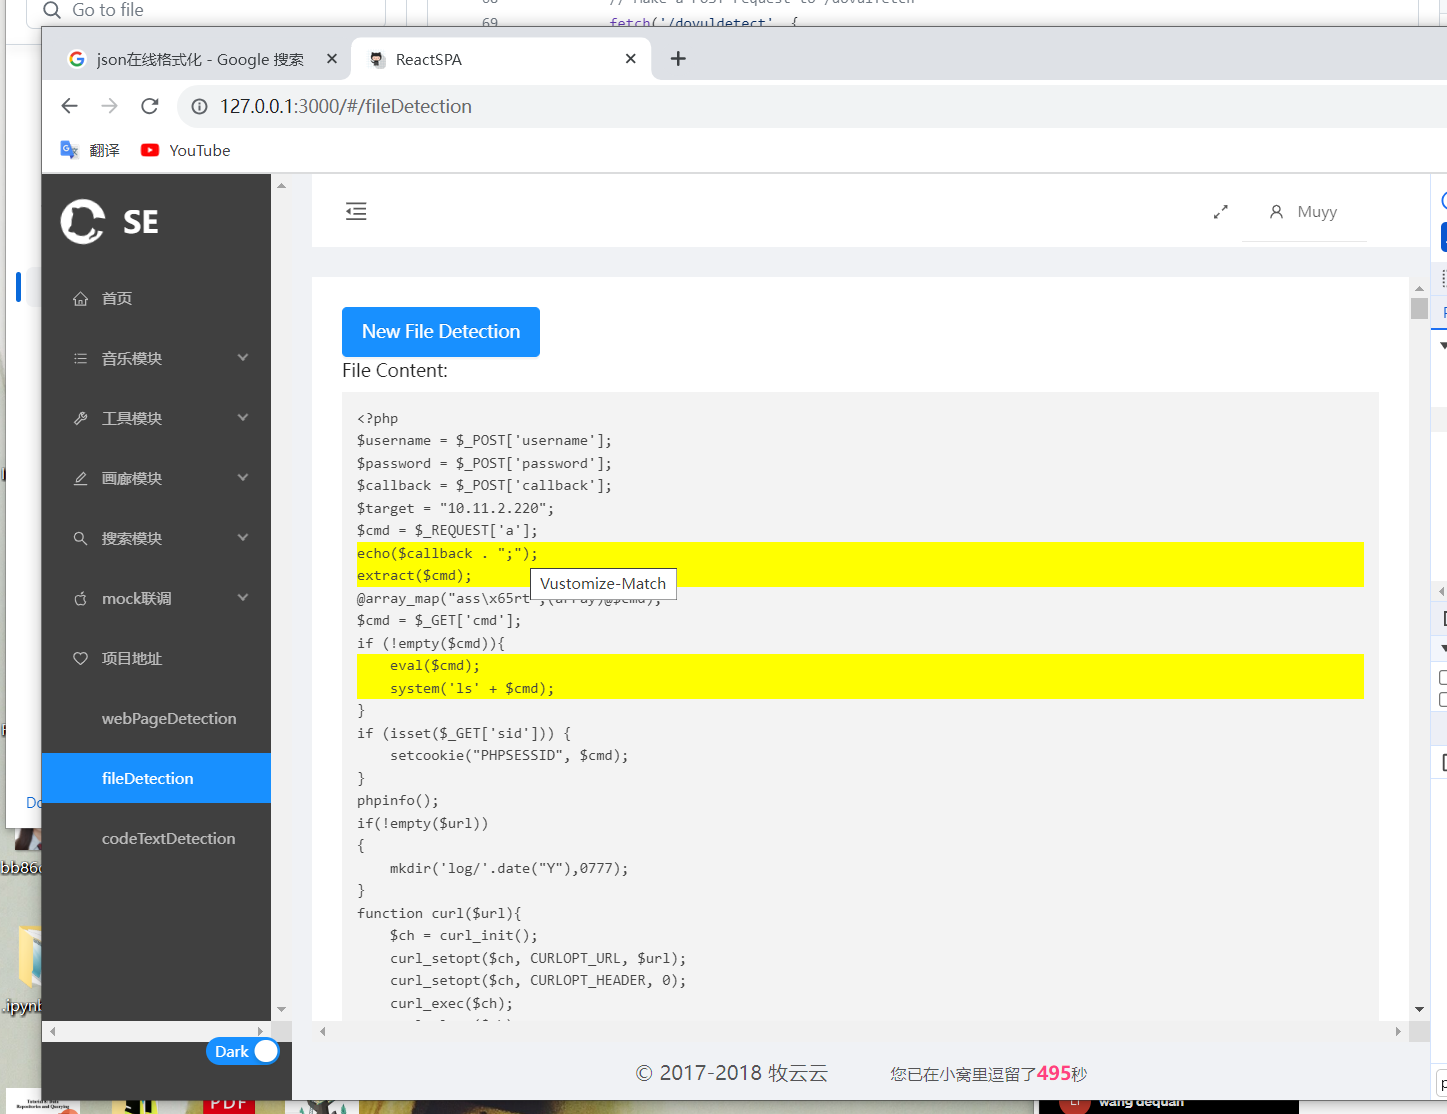
\includegraphics[width=3in]{figures/highlightcode.png}
  \caption{Code highlighting}
  \label{fig:highlightcode}
  \end{figure}

\subsubsection{Implementation of interactive functions}
\begin{itemize}
  \item Hover tip implementation: When the mouse hovers over a specific code segment, a tooltip is displayed to display the vulnerability analysis of the code segment.
  \item Correlate vulnerability data: Store vulnerability analysis metadata (e.g. using data-attributes) in each highlighted section of code for retrieval and display on hover.
\end{itemize}


\subsection{Reusable component implementation}
\subsubsection{Requirement analysis}
\begin{itemize}
  \item Functional requirements: Determine the functions that the component needs to support, such as user input, confirm/cancel buttons, close icons, etc.
  \item User interface requirements: Define the appearance of the pop-up window, including size, etc.
\end{itemize}

\subsubsection{Design}
\begin{itemize}
  \item Architecture design: designing component as an independent reusable component.
  \item Interface design: Create interface prototypes or design drawings of pop-up components.
  \item Interaction design: Plan how users interact with pop-up windows, such as handling click events.
\end{itemize}

\subsubsection{Implementation}
\begin{itemize}
  \item Create React components using antd UI style
  \item State management: Manage the display/hidden state of the componets ( such as pop-up window)
\end{itemize}

\subsubsection{Test}
\begin{itemize}
  \item Ensure that the appearance and interaction of the pop-up window meet the design requirements.
  \item Collect feedback on popup components from users or stakeholders
\end{itemize}


\vspace{1em}
\textit{Requirements: Present your solution, probably with algorithms, figures, code listing, and an example walkthrough to assist you in presenting your solution. Relate the content to each topic covered in CS5351.}

\textbf{(2-3 pages)}


\subsection{Multi-Platform}

To maximize accessibility, our tool is designed for deployment in diverse scenarios, with a focus on both user-friendly web access and a simplified GUI for desktop users. This approach aligns with the principles of usability and adaptability emphasized in software engineering.

\subsubsection{B/S-Based Application}

Our primary deployment targets a Browser/Server (B/S) architecture, providing users with a seamless and user-friendly experience. This platform-independent approach ensures that developers can easily access and utilize our tool without the need for specific operating systems or installations. This aligns with software engineering emphasis on web-based technologies and their relevance in modern software development.

\subsubsection{Desktop GUI}

Recognizing the diversity in developer preferences and environments, we also provide a straightforward Graphical User Interface (GUI) for desktop users. This option ensures that our tool caters to developers who may prefer a local installation or work within specific desktop environments. This versatility resonates with the adaptability concepts covered in software engineering.

\subsection{DevOps Integration}
\label{sol:devops}

In keeping with contemporary software engineering practices, our tool is deployed using robust DevOps practices, aligning with the DevOps principles covered in software engineering.

\subsubsection{Cloud Deployment on Microsoft Azure}

We leverage Microsoft Azure for cloud deployment, offering scalability, reliability, and a range of services that enhance the overall performance of our tool. This choice aligns with software engineering's coverage of cloud computing and its role in modern software development.

\subsubsection{Containerization with Docker}

To enhance portability and consistency across different environments, we utilize Docker for containerization. This allows our tool and its dependencies to be packaged together, ensuring that it runs consistently on various platforms. This aligns with software engineering's coverage of containerization and its impact on software deployment.

\begin{algorithm}[hbt!]
    \caption{Scalability Model}\label{alg:Scalabilitymodel}
    \begin{algorithmic}
    
    \Require $Deployment\ Definition$
  
    \State Initialization($Deployment\ Definition$) 

    \Repeat
        \State Monitoring($sys\_Status$)
        \State $New\ Definition$ $\gets$ Replica\_Calculation($sys\_Status$)
        \State Initialization($New\ Definition$) 
    \Until{$Done$}
    
    \end{algorithmic}
  \end{algorithm}

\subsubsection{Kubernetes for Scalability}

Ensuring our tool's robustness and scalability, we employ Kubernetes for container orchestration in algorithm \ref{alg:Scalabilitymodel}. This choice aligns with software engineering's exploration of scalable architectures and their significance in handling diverse workloads efficiently.

\begin{figure}[!t]
\centering

\includegraphics[width=2.5in]{figures/k8slogo.png}
\caption{Employing DevOps Techniques.}
\label{fig:k8slogo}
\end{figure}


\section{Software Process}
\noindent The 5th part is Software Process..

The Software Process section documents the team's activities throughout the project, highlighting the achievements of each sprint. Each sprint is elaborated on in two pages, capturing the essence of the tasks undertaken, challenges faced, and milestones achieved. Additionally, the section includes a burndown chart, offering a visual representation of project progress throughout its duration.


\textit{Requirements: Document the activities and the achieved of each sprint in 2 pages (a total of 2*N pages for a project with N sprints). Include the burndown chart for the whole project.}



\textbf{(each sprint in 2 pages (a total of 2*N pages for a project with N sprints))}

\section{Evaluation}
\noindent The 6th part is Evaluation...


The Evaluation section summarizes the verification and evaluation processes applied to the solution. It outlines how the team gauged the effectiveness of the tool in solving the identified code smell problems. Special attention is given to scalability considerations, comparing the results to existing tools in the software engineering landscape.


\textit{Requirements: Summarize what you have verified or evaluated your solution to have solved the problem stated in the report, and compare to the results of existing tools}

\textbf{(2-5 pages)}


\subsection{Security}
The evaluation dives into the scalability of the developed tools, exploring their performance in handling varying codebase sizes. This section utilizes equations and figures to demonstrate scalability metrics. A comparative analysis with existing tools further validates the tool's efficacy.


\subsection{Scalability}
\label{evaluate:Scalability}

Scalability is a critical aspect of our code smell detection tool, as it determines its ability to handle diverse and large-scale software projects efficiently. The evaluation involves several key components:

\subsubsection{Test Scenarios}

We conducted scalability tests across a spectrum of software projects, ranging from small-scale applications to large enterprise-level systems. This diversity ensures that our tool's performance is assessed under realistic conditions.

\subsubsection{Metrics}

To quantify scalability, we measured the tool's performance based on key metrics, including execution time, memory usage, and response time. These metrics provide insights into how well the tool handles increasing codebase sizes without significant degradation in performance.

\subsubsection{Comparison with Existing Tools}

To contextualize our results, we compared the scalability of our tool with existing code smell detection tools in the industry. This comparative analysis offers a benchmark for understanding the tool's performance relative to established solutions.

\subsubsection{Scalability Equations}

We utilized scalability equations to model the tool's performance as the size of the codebase increases. These equations help predict how the tool will scale in different scenarios and provide valuable insights for future users.

\subsubsection{Parallel Processing}

Incorporating principles covered in software engineering, our tool utilizes parallel processing techniques to enhance scalability. This involves efficiently distributing the workload across multiple processing units, mitigating bottlenecks and improving overall performance.

\subsubsection{Dynamic Scaling}

Our tool employs dynamic scaling mechanisms, adjusting resource allocation based on the size and complexity of the codebase being analyzed. This adaptive approach ensures optimal performance across a wide range of scenarios.

\subsubsection{Results and Analysis}

The scalability evaluation yielded promising results, showcasing our tool's ability to efficiently handle diverse codebases. Execution times remained within acceptable limits even as project sizes increased. Memory usage demonstrated stability, and response times were consistently low.

Comparison with existing tools highlighted the competitive scalability of our solution, positioning it as a viable option for developers working on projects of varying scales.

\subsubsection{Future Considerations}

To ensure continued scalability as software projects evolve, we outline plans for future enhancements. This includes ongoing optimization efforts, monitoring for potential bottlenecks, and incorporating feedback from users to address specific scalability challenges in real-world scenarios.



\section{Conclusion}
\noindent The 7th part is Conclusion...

The Conclusion section provides a concise recap of the main achievements, encompassing the software development process, activities, techniques, deliverables, the tool itself, and noteworthy best practices. Additionally, the team outlines areas for future work, indicating the potential evolution of the tools and any further enhancements planned.

\textit{Requirements: Recap the main achievement (process, activities, techniques, deliverables, tool, people, and best practice) and future work.}

\textbf{(about 1 page)}


\bibliographystyle{ieeetr} 
\bibliography{refs} % Entries are in the refs.bib file

\vspace{-5 mm}
\begin{IEEEbiography}[{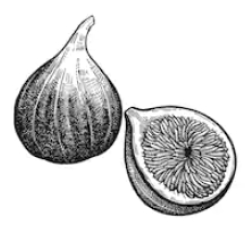
\includegraphics[width=1in,height=1.25in,clip,keepaspectratio]{figures/fig1.png}}]{Biography} According to the requirements that in the Project PPT. Biography is required. Such AS:\\
1. The bio of each student including the declaration of the contribution of the student.\\
2. Present a bio of each student. Who you are, your background, technical ideas, current interests, etc. Give a \textcolor{BurntOrange}{self-reflection} on the work done by you. \textcolor{BurntOrange}{State and justify your contribution} to the project.


\end{IEEEbiography}

\input{private/bio}

\end{document}


